\documentclass[letterpaper,12pt]{article}

\usepackage[table]{xcolor}
\usepackage{threeparttable}
\usepackage{geometry}
\geometry{letterpaper,tmargin=1in,bmargin=1in,lmargin=1.25in,rmargin=1.25in}
\usepackage[format=hang,font=normalsize,labelfont=bf]{caption}
\usepackage{subcaption}
\usepackage{amsmath}
\usepackage{multirow}
\usepackage{array}
\usepackage{delarray}
\usepackage{amssymb}
\usepackage{amsthm}
\usepackage{lscape}
\usepackage{natbib}
\usepackage{setspace}
\usepackage{float,color}
\usepackage[pdftex]{graphicx}
\usepackage{pdfsync}
\usepackage{verbatim}
\usepackage{placeins}
\usepackage{geometry}
\usepackage{pdflscape}
\synctex=1
\usepackage{hyperref}
\hypersetup{colorlinks,linkcolor=red,urlcolor=blue,citecolor=red}
\usepackage{bm}


\theoremstyle{definition}
\newtheorem{theorem}{Theorem}
\newtheorem{acknowledgement}[theorem]{Acknowledgement}
\newtheorem{algorithm}[theorem]{Algorithm}
\newtheorem{axiom}[theorem]{Axiom}
\newtheorem{case}[theorem]{Case}
\newtheorem{claim}[theorem]{Claim}
\newtheorem{conclusion}[theorem]{Conclusion}
\newtheorem{condition}[theorem]{Condition}
\newtheorem{conjecture}[theorem]{Conjecture}
\newtheorem{corollary}[theorem]{Corollary}
\newtheorem{criterion}[theorem]{Criterion}
\newtheorem{definition}{Definition} % Number definitions on their own
\newtheorem{derivation}{Derivation} % Number derivations on their own
\newtheorem{example}[theorem]{Example}
\newtheorem{exercise}[theorem]{Exercise}
\newtheorem{lemma}[theorem]{Lemma}
\newtheorem{notation}[theorem]{Notation}
\newtheorem{problem}[theorem]{Problem}
\newtheorem{proposition}{Proposition} % Number propositions on their own
\newtheorem{remark}[theorem]{Remark}
\newtheorem{solution}[theorem]{Solution}
\newtheorem{summary}[theorem]{Summary}
\bibliographystyle{aer}
\newcommand\ve{\varepsilon}
\renewcommand\theenumi{\roman{enumi}}
\newcommand\norm[1]{\left\lVert#1\right\rVert}

\definecolor{myYellow}{HTML}{F8D58B}
\definecolor{myBlue}{HTML}{CBE7F9}


\begin{document}

\begin{spacing}{1.5}


\title{Figures for Florida interactive map of data center land article}

\maketitle

\section{Introduction}\label{SecIntro}


\begin{figure}[htbp]\centering \captionsetup{width=3.0in}
  \caption{Screenshots of Florida interactive map of available data center land under SB 484}
  \label{Fig1_MainFig}
  % First panel
  \begin{subfigure}[b]{0.49\textwidth}
      \centering
      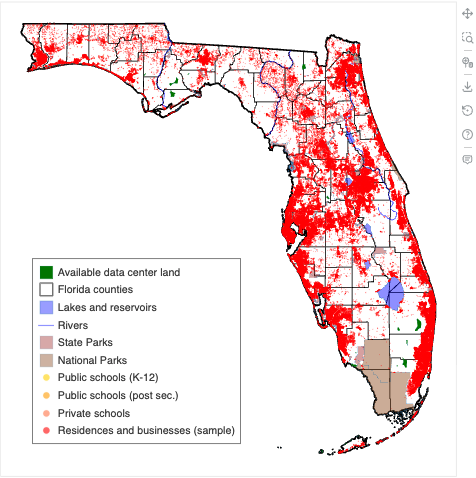
\includegraphics[width=\textwidth]{./images/FL_MapMain.png}
      \caption{All layers}
      \label{Fig1_MainFigA}
  \end{subfigure}
  \vfill % Adds vertical space between the subfigures
  % Second panel
  \begin{subfigure}[b]{0.49\textwidth}
      \centering
      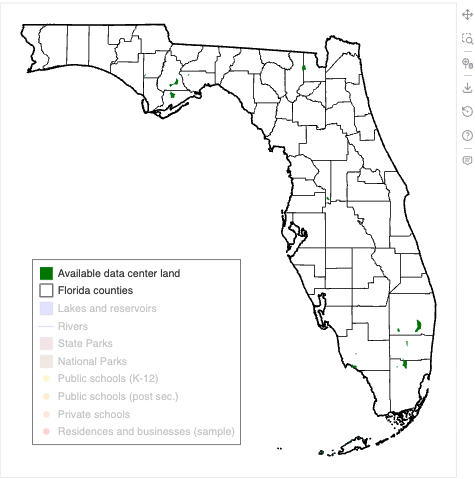
\includegraphics[width=\textwidth]{./images/FL_MapClean.png}
      \caption{Highlighting available data center land}
      \label{Fig1_MainFigB}
  \end{subfigure}
  \caption*{\footnotesize{Source: Richard W. Evans (@RickEcon) updated Mar. 17, 2026. Note that the business and residence scatter points are a random sample of 200,000 centroid points from the over 7 million residences and businesses in the data. I used the full sample of business and residence outlines in the calculation for available data center land, but I excluded the majority of those points from this figure in order to successfully plot them.}}
\end{figure}


\end{spacing}

\end{document}
